\subsection{Transient Response Analysis}
\begin{figure*}[tph]
    \centering
    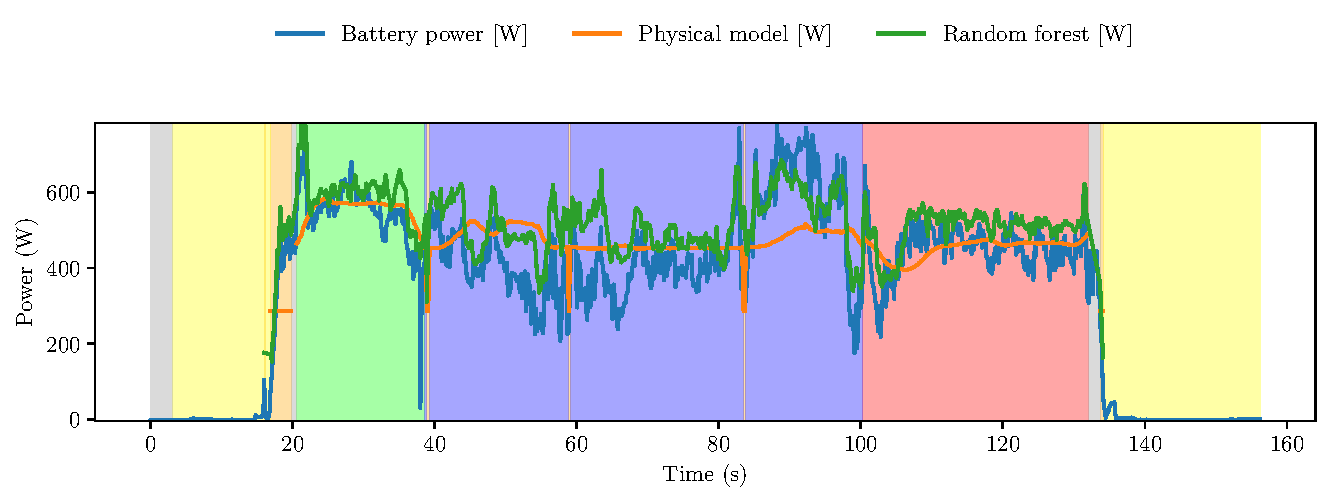
\includegraphics[width=0.9\linewidth]{figures/phases_power_compare.pdf}
    \caption{Dynamic (transient) response of both models versus real-time power consumption during flight 79. Flight segments are colored by flight phase as per legend in Figure \ref{fig:phase_seg_01}.}
    \label{fig:phase_power_comp}
\end{figure*}
To assess the models’ ability to capture short-term power dynamics, the predicted and measured power trajectories of the representative flight $79$ are compared in Figure~\ref{fig:phase_power_comp}. The time series spans critical operational phases—taxi, climb, cruise, descent, and hover—providing a detailed view of model behavior during transitions and high-dynamic maneuvers. Measured power exhibits pronounced fluctuations during climb and cruise, driven by rapid changes in thrust, drag, and control inputs. The physics-based model generates smooth, continuous predictions that follow the general trend but consistently lags behind or underestimates transient peaks and dips, indicating a limited ability to respond to sudden changes. In contrast, the Random Forest model closely tracks the measured power across all phases, accurately replicating rapid variations in response to flight dynamics and environmental conditions. This superior temporal fidelity highlights the model’s strength in learning complex, time-varying interactions from historical data. Unlike analytical models constrained by fixed equations, the Random Forest approach adapts to real-world nuances such as control effort, wind gusts, and maneuver intensity. These findings underscore a key advantage of data-driven methods: their capacity to model transient behavior and operational subtleties that are difficult or impossible to encode in physics-based formulations. 

\subsection{Quantitative Performance Comparison}

Now, the two models—Random Forest and the physics-based model—are evaluated using standard error metrics: MAE, RMSE, and MAPE. As illustrated in Figure~\ref{fig:model_comp}, the Random Forest model achieves a consistent improvement of approximately 45–50\% across all metrics compared to the physics-based approach. 
\begin{figure}[h]
    \centering
    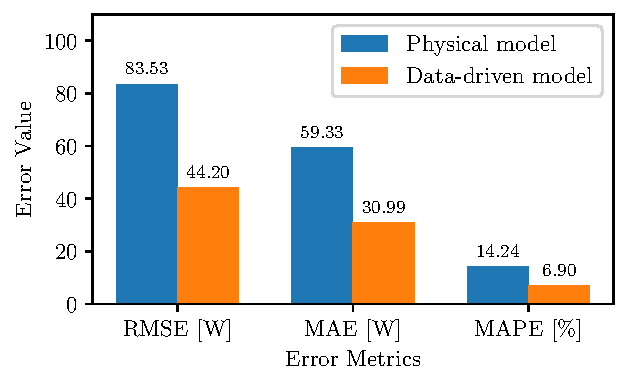
\includegraphics[width=0.9\linewidth]{figures/model_comparison.pdf}
    \caption{Performance comparison of the two models based on various error metrics.}
    \label{fig:model_comp}
\end{figure}
This substantial gain aligns with recent findings in the literature \cite{zhang2021}, which emphasize the inherent limitations of physics-driven models in complex, real-world scenarios. While such models can capture broad trends in power consumption based on aerodynamic and propulsion principles, they often fail under dynamic flight conditions due to simplifying assumptions, unmodeled nonlinearities, and sensitivity to parameter uncertainty \cite{dorling2017}. In contrast, the Random Forest model, trained on a large dataset of real flight observations, effectively learns the intricate, non-linear dependencies between flight states (e.g., speed, acceleration, payload) and energy demand. This data-driven capability enables significantly higher prediction accuracy, particularly in variable or high-dynamic regimes. The results reinforce the growing consensus that machine learning methods outperform traditional physics-based models in terms of numerical precision and robustness, making them better suited for accurate energy estimation in practical UAV operations \cite{muli2022}.


\subsection{Interpretability and generalisation}
Interpretability refers to the degree to which the influence of input variables on model predictions can be understood and explained. Physics-based models are grounded in well-established analytical equations derived from fundamental principles of aerodynamics, mechanics, and thermodynamics. This inherent transparency allows for direct physical interpretation of model outputs. In contrast, Random Forest model, comprising ensembles of decision trees, operate through complex, non-linear statistical learning processes. While feature importance analysis can provide partial insight into which inputs most influence predictions, the internal decision logic remains opaque and difficult to trace. As a result, data-driven models offer only moderate interpretability, limiting their utility in safety-critical applications where explainability is paramount \cite{zhang2021, muli2022, gora2022}.

Generalization is the ability of a model to maintain accuracy when applied to unseen flight conditions or new UAV platforms. It is a critical factor in real-world deployment. To evaluate this, we conducted a sensitivity test by modifying the linear acceleration of a representative flight beyond the range observed in the training data. The resulting energy consumption (calculated according to Eq. \ref{eq:energy}) trend is shown in Figure~\ref{fig:generalisation}, where the Random Forest model incorrectly predicts a decrease in energy consumption with increasing acceleration. This is an unphysical behavior. This contrasts sharply with the expected trend observed within the training regime (Figure~\ref{fig:energy_vs_az}), where energy consumption increases with acceleration, consistent with real-world dynamics. The model’s erroneous extrapolation highlights a key limitation: Random Forests lack the ability to generalize reliably outside the domain of their training data. 

\begin{figure}[h]
    \centering
    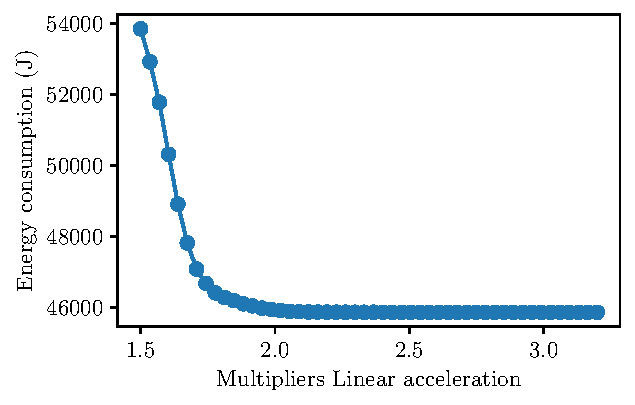
\includegraphics[width=0.9\linewidth]{figures/Energy_vs_az_generalisation.pdf}
    \caption{Sensitivity of ML model to linear acceleration values outside the training data range.}
    \label{fig:generalisation}
\end{figure}
Both physics-based and data-driven models exhibit strong performance when operating within the range of conditions present in their training data \cite{zhang2021}. Physics-based models may require manual recalibration of physical parameters (e.g. drag coefficients, motor efficiency) when applied to different platforms or environments \cite{hwang2018}. Similarly, data-driven models often fail to extrapolate correctly and may produce physically implausible results when pushed beyond their training boundaries. These findings underscore a fundamental trade-off: while physics-based models offer superior interpretability, and data-driven models deliver higher accuracy within their domain, neither approach ensures robust performance across all operational scenarios without additional adaptation. 
